
%----------------------------------------------------------------------------------------

\section{`Small Data' Infrastructure}

\begin{sectionframe} % Custom environment required for section slides
	\frametitle{`Small Data' Infrastructure}
	%\framesubtitle{Subtitle}

% 	Some section slide content

% 	This is on another line
\end{sectionframe}

%----------------------------------------------------------------------------------------



\begin{frame}{`Small data' research}
 \begin{figure}[H]
    \centering
        \vspace{-0.5cm}
        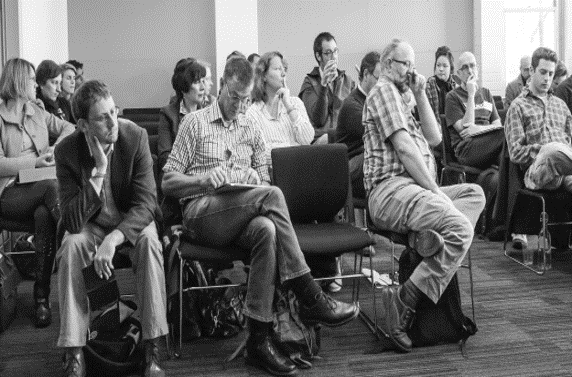
\includegraphics[height=.725\textheight]{figures/Archaeologists-standards.png}
        \caption{Archaeologists contemplate data standards (FAIMS Stocktaking, 2012)}
        \label{fig:figure7}
 \end{figure}
\end{frame}

%----------------------------------------------------------------------------------------

\begin{frame}{Context: the challenge of `small data'}
    `Long tail' research: most field data is small data \parencite{Borgman2015-rh}
    \begin{itemize}
        \item Smaller scale
        \item Diverse approaches
        \item Heterogeneous data
        \item Data and infrastructure emerge from fieldwork. 
        \item Relative lack of standards.
        \item Limited funding.
        \item Large(r) new data streams make everything harder.
        % \item Challenges associated with big(ger) data from photogrammetry, SfM, video, geophysics, etc., will exacerbate these problems.
    \end{itemize}
\end{frame}

%----------------------------------------------------------------------------------------


\begin{frame}{The data lifecycle}
 \begin{figure}[H]
    \centering
    \vspace{-0.5cm}
        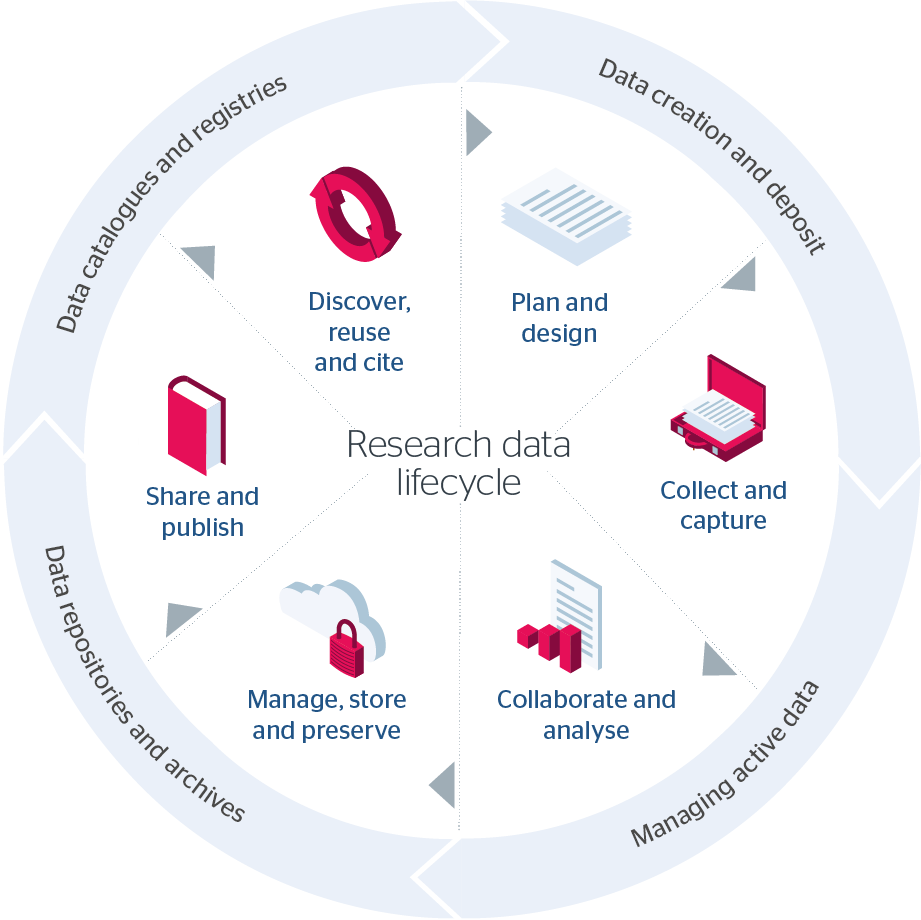
\includegraphics[height=.75\textheight]{figures/research-data-life-diagram.png}
        \caption{\cite{Jisc2018-gx} Image CC-BY-ND}
        \label{fig:figure9}
 \end{figure}
\end{frame}

%----------------------------------------------------------------------------------------


\begin{frame}{Infrastructure across the data lifecycle}
    Three main phases of the data lifecycle
    \begin{itemize}
        \item Publication (most mature)
        \item Processing and analysis (less mature) \parencite{Stewart_Lowndes2017-lj, Alveo2019-tk} .
        \item Capture (least mature and least supported by `normal' tools) \parencite{Bureau_of_Reclamation2017-xl}.
    \end{itemize}
\end{frame}
\textbf{}